\subsection{Why physically contiguous memory is needed}

\begin{frame}
  \frametitle{The mighty MMU}

  \begin{itemize}
  \item Modern CPUs have MMU.
    \begin{itemize}
    \item Virtual $\rightarrow$ physical address.
    \end{itemize}
  \item Virtually contiguous $\notimplies$ physically contiguous.
  \item So why bother?
  \end{itemize}
\end{frame}

\begin{frame}
  \frametitle{System devices}

  \begin{itemize}
  \item MMU stands behind CPU.
  \item There are other chips in the system.
  \item Some require large buffers.
    \begin{itemize}
    \item 5-megapixel camera anyone?
    \end{itemize}
  \item On embedded, there's plenty of those.
  \end{itemize}
\end{frame}

\begin{frame}
  \frametitle{The mighty DMA}

  \begin{itemize}
  \item DMA can do vectored I/O.
  \item Gathering buffer from scattered parts.
  \item Contiguous for the device $\notimplies$ physically contiguous.
  \item So why bother?
  \end{itemize}
\end{frame}

\begin{frame}
  \frametitle{The mighty system MMU}

  \begin{columns}[c]

    \column{.5\textwidth}
    \begin{itemize}
    \item What about a~system MMU?
      \begin{itemize}
      \item Address coming from the device $\rightarrow$ physical
        address
      \end{itemize}
    \item Same deal as with CPU's MMU.
    \item So why bother?
    \end{itemize}

    \column{.5\textwidth}
    \begin{center}
      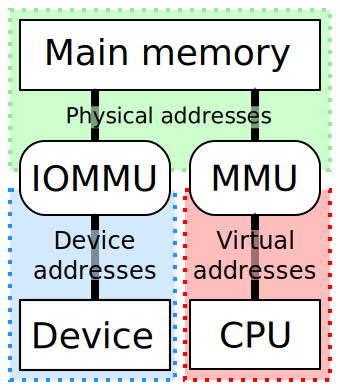
\includegraphics[width=\textwidth]{build/iommu-vs-mmu.eps}
    \end{center}

  \end{columns}
\end{frame}

\begin{frame}
  \frametitle{Cost, speed \& power}

  \begin{itemize}
  \item Every chip costs.
    \begin{itemize}
    \item Money and power.
    \end{itemize}
  \item More complex chips cost more.
  \item Not all systems have DMA with SG or system MMU.
  \item System MMU takes time.
  \end{itemize}
\end{frame}
